\chapter{Motivations for key-finding}
\label{chap:chap50}

\begin{quote}
    Why does key-finding matter? Give examples of questions one could ask of a symbolic corpus that require key identification. [3-5 pages]
\end{quote}
\clearpage

% Across the literature, the most mentioned application of key-finding algorithms is its use in \emph{harmonic mixing} applications for DJs.
% There are companies that value accurate and automatic annotations of the musical key for this purpose.
% However, as described in audio feature taxonomies, a musical key is also a feature that characterizes a musical fragment.
% Its presence (tonal music) or absence (modal or atonal music), its strength (highly harmonic vs. highly contrapuntal), and its change over time (intermediate keys, modulations) can tell us valuable information about a piece of music and its characteristics.
% When analyzed from a multitude of viewpoints, it has been shown by Sapp that different music create very different tonal visualizations, or as he calls them, \emph{keyscapes}.

% We refer to key-finding as the process of determining the key of a musical piece, for example, the key that is written on the title of the piece.

% Furthermore, a key-finding model is an algorithm that allows us to determine that key automatically given a digital representation of the piece of music (see Question \ref{chap:chap4} for a more extensive review of digital representations of music).

% Over the years, multiple applications have emerged for these type of systems. These applications can be divided in the applications of \emph{global} key-finding algorithms and \emph{local} key-finding algorithms (see Question \ref{chap:chap6} for a further discussion on global and local keys).

% \todo[inline]{Locate applications based on the papers for this question}

% \subsection{Global key-finding applications}

% Some of the utilities of key-finding algorithms are music classification, music cataloguing, and harmonic mixing for DJs.

% These applications appear frequently across the literature of key-finding models.

% \subsection{Local key-finding applications}

% Although not as frequently mentioned as the applications of global keys, researchers have also found useful applications for local key-finding models across the field of Music Information Retrieval.
% \begin{enumerate}
%     \item Structural segmentation of the music
%     \item Roman numeral analysis
%     \item Pitch-spelling algorithms
%     \item Chord labeling
%     \item Visualizing tonality in music
% \end{enumerate}

% % One problem that most of these applications of local key-finding models share is that local keys are very difficult to evaluate quantitatively, that is, empirically, we know that keys are related with chords, the spelling of the notes, functional harmony, and musical structure, but we do not know how much and that is very difficult to know

% Local key-finding models and their applications are, nevertheless, less common. Mainly, because local key-finding models are very difficult to evaluate. On the other hand, global key-finding models are relatively easier to evaluate quantitatively, and have become more popular over the years.

% \subsection{Going further into new research questions}

% Sapp \cite{sapp2011computational} studied tonality through the computation of a key-finding model at different window lengths of a piece of music.

% From the tonal regions obtained, he categorized different regions as either chords, tonicizations, and modulations.

% How do we know this is true?

% \begin{figure}[h]
%     \centering
%     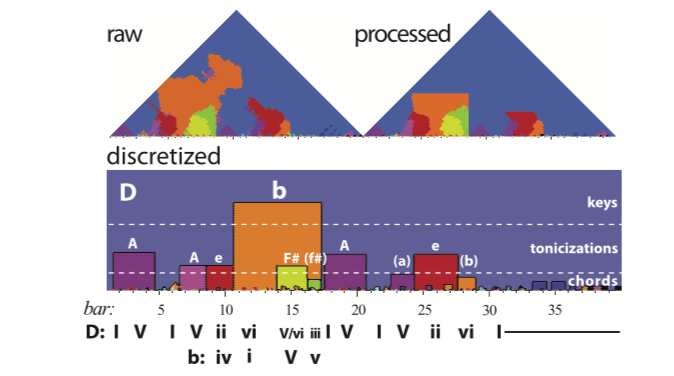
\includegraphics[width=0.6\textwidth]{figures/Q5_1.png}
%     \caption{Key-finding algorithm used to delimit chords, tonicizations, and modulations in a piece of music}
%     \label{fig:Q5_1}
% \end{figure}

% \subsection{Concrete questions that we can ask in a symbolic music corpus}

% How many changes of key (modulations) happen in a given piece?
% How many tonicizations happen in a given piece?
% How many of those would be annotated by a human annotator?
% How many of those overlapped or mismatched between annotators?
% How many of those were found by local key-finding algorithms?
% How many of those end in a Perfect Authentic Cadence or confirm other structural cues mentioned in music theory for modulations?
% How many times does the local key mismatches the global key of the beginning of the piece?
% How many times does the local key mismatches the global key of the end of the piece?

% \subsection{Interesting properties of musical keys in the study of tonality}

% What does evaluation has to do with any of this? I should be really talking about applications.

After the first attempt of designing a key-finding algorithm by Longuet-Higgins \cite{longuethiggins1971interpreting}, many algorithms have followed throughout the years. These algorithms, using different approaches and methodologies, attempt to retrieve the key of digital music representations in the symbolic and audio domains (see Question \ref{chap:chap3} for a survey on key-finding models). 

The problem of designing an algorithm that is able to retrieve musical keys, among other tonal features, has also been the motivation of several dissertations \cite{gomez2006tonal, campbell2010automatic, korzeniowski2018harmonic, sapp2011computational, chew2000towards}. 

During the research literature, the applications for key-finding models are often discussed and a few examples are frequently mentioned: the possibility of indexing large volumes of music by their musical key in digital music libraries; the automatic annotation of music data available on the web, which does not usually include the annotation of the musical key; and the reliable extraction of musical keys as machine learning features, which have been shown to be useful in other Music Information Retrieval (MIR) tasks \cite{mauch2010approximate, chai2005detection}. Another application, particularly interesting for those pursuing the commercial viability of key-finding models, comes surrounding certain music communities, for example, Electronic Dance Music (EDM), where the knowledge of the key can be very helpful for performers during the mixing process, given that a common technique involves mixing music with similar harmonic structures, a technique known as \emph{harmonic mixing}. This necessity opens a commercial opportunity for the designers of key-finding models, given that companies profit from having reliable annotations that they can offer to their users. 

Nevertheless, aside from the necessity of key-finding models in digital libraries and commercial applications, researchers have also encountered themselves (maybe as a byproduct of research and design decisions), with interesting musicological questions. Here, I decide to concentrate on those, formulating a few questions based on the research inquiries, claims, and assumptions that can be found surrounding the literature of key-finding algorithms.\footnote{Unless explicitly mentioned, the questions listed here are not direct quotes from the cited papers but questions formulated given a---sensible---interpretation of the statements in the cited papers. Following the question, comes a discussion of the paper (and the context) from which the question was formulated.}

\section{Questions regarding the study of key-finding algorithms}

\textbf{\emph{What is the field that studies musical keys and tonality?}}

According to Vos \cite{vos2000tonality}, there is a natural ``bias'' in the scientific study of tonality, due to the interdisciplinarity of the problem and the fact that no person is specialized in music theory, music history, psychoacoustics, music psychology, and computer science. All at the same time. If there is a person with such a background, certainly the expertise in each area is asymmetrical, which leads to a biased view of the problem towards the area where the researcher has more expertise. This has a noticeable effect in the research of key-finding algorithms, as a successful algorithm for finding musical keys \cite{korzeniowski2018harmonic}  could reduce its discussion on musical implications of keys, tonality, harmonic tension, and ambiguity to a negligible part of the research document, completing the rest of the document with thorough, well-designed experiments of machine learning and statistical analysis, typical of computer science but difficult to find in any music-theoretical study. Krumhansl revisits this issue \cite{krumhansl2004cognition}, surveying studies from multiple disciplines that try to explain what tonality is (musical keys included), according to different perspectives. In that study, Krumhansl dedicates a section to discuss the point of view of music cognition, acoustics, musicology, computer science, music theory, and brain science. 

In a very different---almost comedic---work, Aucouturier and Bigand also touch on the issues of interdisciplinarity \cite{aucouturier2012mel}.

\textbf{\emph{Can we use key-finding algorithms as ``debugging'' tools for testing music theories? For example, can we use them to observe the difference between a modulation and a tonicization?}}

In his dissertation, Sapp introduced the \emph{keyscapes} \cite{sapp2011computational}, which allow the computation of key-finding algorithms at different window sizes in a music score and, moreover, visualizing the resulting output. He claims that such visualization techniques can be useful as evaluation tools, for example, by visually assessing the strengths and weaknesses of a particular algorithm. Additionally, Sapp claims that such visualization tools can also be used to find the distinction between a modulation and a tonicization, as tonicizations (in his proposed visualization technique) do not extend towards the top end of the \emph{keyscape}, while true modulations do. This brings an interesting point, as there is no easy way to quantitatively distinguish a modulation from a tonicization, however, claiming that such visualization tools can do it opens up the door to further musicological inquiries about the concepts of modulation and tonicization, and their scientific evaluation. 


\textbf{\emph{When did tonality ``start''? And, did the establishment of ``tonal music'' had something to do with the refinement of temperament?}}

In the same paper discussed previously \cite{vos2000tonality}, Vos argues that one of the root causes in the ``fuzziness'' of the term \emph{tonality} and what it refers to, is that there is no clear boundary of when and where that term should be applied historically. He claims that tonality may be found in medieval folk songs and Palestrina's ``modal counterpoint'', and at the same time, examples by Bach can be interpreted as ``modal music''. If that is true, how can we know whether the data used for training and testing key-finding models is an accurate representation of \emph{tonal} music explained by a major or minor key.

In a different statement, Vos argues that one factor that could have contributed significantly to the establishment of "tonal music" is the refinement of temperament in the 18th century. Temperament \emph{incentivized} modulation and became a norm in Bach and subsequent composers. If used for analyzing a representative sample of music compositions, a reliable local-key-finding algorithm could be used for addressing this question.

\textbf{\emph{Can we use key-finding evaluations as a metric to evaluate the capability of spatial representations of music?}}

In her dissertation \cite{chew2000towards}, Chew introduced a spatial representation of tonality, which consists of multiple dimensions and allowed the computation of keys and chords by locating them in such tonal space. This approach has been followed by other researchers who have proposed other spatial representations of tonality \cite{harte2006detecting}. Such representations are very difficult to assess by humans, however, using computational approaches to predict the key or chords in a musical excerpt could be a useful way of measuring their validity. This encourages the collection and annotation of data, which is the same data used for designing and evaluating key-finding algorithms. Additionally, having a reliable spatial representation of tonality would mean understanding better how tonality works. 

\textbf{\emph{Does having the knowledge of the key changes throughout a musical piece reveal the structure of the piece?}} 

In their study, Chai and Vercoe \cite{chai2005detection} found that in the self-similarity matrix of a piano sonata by Mozart, with no apparent repetitions, the repetitions became obvious as soon as the information of key changes were introduced. Of course, this information would not always yield favorable results, but it could help finding structure in certain musical forms, like sonata-allegro movements.

\textbf{\emph{Can the frequency of chords inform us about the relationship between chords and keys?}}

Using the chord frequencies annotated in Budge's dissertation \cite{budge1943study}, Bellmann \cite{bellmann2006about} designed a \emph{key profile} to be used with a new key-finding algorithm. The resulting key-finding algorithm outperformed the accuracy of the Krumhansl-Schmuckler algorithm \cite{krumhansl1990cognitive}, using solely information about chord progressions.

Regarding how the key-finding algorithms should process the musical inputs, Quinn has explicitly pointed out a few questions that, through observation, seem as much of a musicological nature as they seem of an engineering nature \cite{quinn2010are}. Quinn considers that these questions ``dominate'' the key-finding literature and the choices done by researchers on the field: ``\textbf{\emph{Should window size be defined in terms of chronological time, notational (metrical) time, or number of note onsets? How big should the window be? How does key-finding for a given window take into account results for previous windows? How should pitch-class distributions be weighted? How is a key determination made from a given pitch-class distribution?}}''

Finally, in a data-driven study by White and Quinn \cite{white2018chord}, a Hidden Markov Model (HMM) was given the freedom to learn harmonic functions from Bach chorales, examples of the Kostka-Payne harmony textbook, and the McGill Billboard dataset. This process followed mostly an unsupervised approach, without the explicit involvement of the human experts deciding which functions needed to be learnt by the model. As a result, the model came up with different architectures for each type of music, sometimes defying the expectations of music theory, and sometimes, at least partially, validating them. This poses the following question: \textbf{\emph{can we use key-finding and chord recognition models, to propose new music theories?}}

\bibliographystyle{plainnat}
\bibliography{zoterorefs}